\section{Crowdfunding}

Si tratta di un \textit{finanziamento dal basso}, ovvero ``dal popolo''. È
spesso un'attività associata alle start-up, in quanto non hanno una grande
disponibilità di capitali, anche se non costituiscono un veicolo di
finanziamento, a meno di non proporre un proprio prodotto tramite la
piattaforma. Esistono però anche grosse aziende che lo fanno, più che altro per
capire se il prodotto che deve essere venduto può essere di un qualche interesse
o meno. Le attività di crowdfunding non danno solo denaro, ma offrono anche
visibilità. Il capitale che viene offerto non è legato alla società, ma è legato
al progetto. Solitamente la persona che offre i propri soldi riceve in cambio un
prodotto, spesso tangibile e concreto, creando quindi un sistema di
\textit{pre-booking}.

Ci sono pochi esempi di crowdfunding nei quali in cambio vengono date quote a
chi partecipa. Queste sono molto complesse (quale percentuale dell'azienda
cedere in base ad una certa quantità di denaro?) e al momento non ci sono
ancora track record positivi.

\subsection{Caratteristiche}

Nel crowdfunding è molto spesso importante creare prodotti ``speciali'',
invogliando l'utente ad acquistare i prodotti e finanziare il progetto. Anche
la comunicazione mediatica è fondamentale: è importante postare foto, notizie e
aggiornamenti sull'andamento del progetto: persone importanti o affermate nel
campo spesso possono costituire un fattore importante per aumentare possibili
investimenti\footnote{Il \textit{track record} di una persona è quindi
importante}. La credibilità del team è fondamentale: non c'è nessuna garanzia
che, al raggiungimento della soglia minima, quei soldi vengano effettivamente
usati per il progetto. Più alta è la reputazione delle persone coinvolte
maggiore è la probabilità che quel progetto sia serio.

Spesso i siti che hostano i progetti crowdfunding hanno una trattenuta sulla
somma finale raccolta.

In caso il crowdfunding non raggiunga la soglia minima i soldi non vengono
prelevati dal conto delle persone, ma vengono restituiti.

\section{Come le start-up falliscono}

Quante start-up falliscono? Fornire un numero è difficile: la mortalità delle
start-up è alta nelle prime fasi, per poi calare (anche brutalmente) verso le
ultime fasi. Questo perché la struttura dell'azienda stessa migliora, ed è più
difficile che il progetto fallisca quando ci sono degli investitori che ci
tengono al fatto che i propri soldi non vengano ``sprecati''.

Ma come mai le start-up falliscono? Esistono diverse ragioni per ciò:
\begin{itemize}
 \item Errata analisi di mercato
 \item Concorrenza
 \item Non è presente abbastanza marketing
 \item L'MVP è troppo povero e non suscita interesse al mercato
\end{itemize}

\subsection{Top 20 cause di fallimento start-up}

Queste sono, in ordine decrescente:
\begin{enumerate}
 \item \textbf{Ignore customers}: è importante ascoltare i clienti e non
 sottovalutare le loro richieste, cosa che capita spesso ai ``tecnofili''.
 Altro aspetto tipico di quest'ultimi è sopravvalutare le capacità del mercato
 di assorbire il loro prodotto e la capacità dell'utente medio di imparare ad
 usarlo. Un altro aspetto da non sottovalutare è dare per scontato che gli
 utenti abbiano i miei stessi interessi.
 \item \textbf{No market need}: capire quando e se il mercato richiede un certo
 prodotto è fondamentale: questo errore è più grave del precedente, nel quale
 si ignora la direzione più giusta da intraprendere, in quanto non si ascoltano
 né i feedback del mercato, né è stata fatta una buona analisi di mercato a
 priori.
 \item \textbf{Not the right team}: uno degli elementi critici nella vita delle
start-up è la qualità del team. Le 5 cose importanti per le start-up sono:
\begin{itemize}
 \item il prodotto
 \item il mercato
 \item il team
 \item il team
 \item il team
\end{itemize}
  È quindi fondamentale avere un team efficiente che funzioni alla perfezione,
soprattutto sotto stress. La motivazione rischia di calare presto, e con questo
i litigi possono esplodere facilmente. In una start-up non è possibile lavorare
da solo, ma è necessario il team.
 \item \textbf{Poor marketing}: ho un prodotto ma non lo so vendere
 \item \textbf{Ran out of cash}: come mai hanno finito i soldi? In quanto si
 fanno uno degli errori elencati sopra
 \item \textbf{Need biz model}
 \item \textbf{Product mis-timed}
 \item \textbf{Lack passion}
 \item \textbf{Failure to pivot}
 \item \textbf{Poor product}
 \item \textbf{Pricing issues}
 \item \textbf{Don't use the network}
 \item \textbf{Disharmony on team}
 \item \textbf{Lose focus}
 \item \textbf{Burn out}
 \item \textbf{Get outcompeted}
 \item \textbf{No financing}
 \item \textbf{Bad location}
 \item \textbf{Only part-timed}
 \item \textbf{Bad time to start}: magari il prodotto è interessante, ma si
 comincia con un brutto tempismo, o magari quando il mercato non è pronto
\end{enumerate}

\begin{figure}[t]
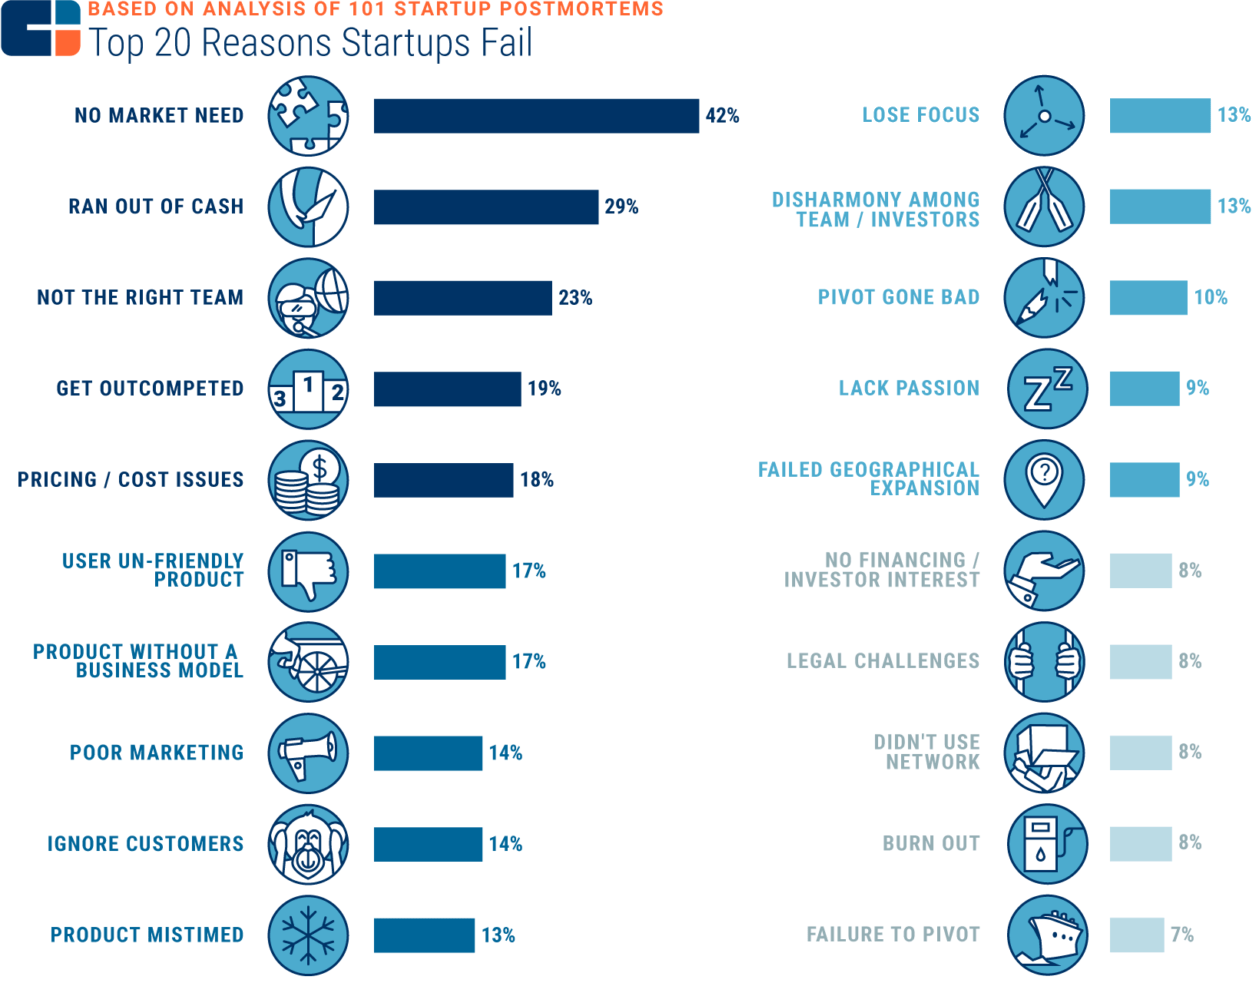
\includegraphics[scale=0.3]{chartFailureStartup}
\caption{Lista dei top 20 motivi di fallimento di una startup}
\end{figure}

Altre informazioni riguardo alle ragioni di fallimento di una startup si possono
trovare al link:
\url{https://www.cbinsights.com/research/startup-failure-reasons-top/}
Nessuna delle voci citata, come vediamo, è legata all'idea.

\subsection{Annunci sponsorizzati vs annunci organici}

Gli annunci \textbf{sponsorizzati} sono quelli per cui si paga, mentre quelli
\textbf{organici} sono quelli determinati dall'algoritmo di ricerca e si
piazzano dopo i primi.

\textbf{Pay-per-click}: in base a delle parole di ricerca, un'azienda può pagare
affinché il suo sito compaia in un annuncio sponsorizzato. Se ci sono più
aziende interessate a ottenere visibilità in base alle stesse parole di
ricerca, si apre un'asta e i posti più in alto vanno (ovviamente) al migliore
offerente.

Ogni annuncio ha un budget associato che diminuisce a ogni click.

Le aziende che dipendono dall' e-commerce fanno grossi investimenti in adwords.

\section{L'idea in una start-up}

Per idea di una start-up s'intende il concetto che sta dietro al prodotto che
si vuole creare. Normalmente le start-up nascono da un'idea, ma non è l'idea in
sé l'importante, ma come la si realizza\footnote{Come ha detto Thomas Edison:
\emph{``1\% inspiration, 99\% perspiration''}, sottolineando come dietro un'idea
ci sia moltissimo lavoro da fare.}. Spesso, infatti, non è l'idea a mancare
(o a non essere valida), ma manca l'approccio al mercato, al cliente, al
business o la capacità di esecuzione dell'idea.

\section{Investitori}

Un investitore cosa guarda in una start-up per capire se investirci oppure no?
Come già detto, nelle prime fasi viene il team, ma in generale, sono presenti
\textbf{quattro elementi} che vengono guardati in assoluto per capire se
investire:
\begin{itemize}
 \item \textbf{Redditività}: gli investitori si aspettano di ottenere, con un
 investimento molto precoce ed ad altissimo rischio, un altissimo guadagno. Al
 contrario, gli investitori che investono nelle start-up mature hanno un basso
 ritorno, ma è anche vero che ci sono dei bassi rischi.
 \item \textbf{Fattibilità}: bisogna capire se il prodotto è fattibile (in
 generale) e se il nostro team è in grado di farlo.
 \item \textbf{Scalabilità}: indica la velocità di crescita. È una delle cose
 che le start-up, soprattutto digital, dovrebbero avere. Un progetto può essere
 a crescita lineare o esponenziale. Si definisce a crescita \textbf{lineare}
 nel caso in cui per aumentare i guadagni devo aumentare in maniera
 proporzionale gli investimenti. In certi casi la crescita della società è
 lineare per natura dell'azienda stessa. Si parla, invece, di crescita
 \textbf{esponenziale} nel caso in cui i guadagni aumentino in maniera
 esponenziale, indipendentemente (o quasi) rispetto ad una crescita lineare
 degli investimenti fatti (ad esempio i libri o le app sono prodotti scalabili).
 Prodotti non scalabili sono quelli dove è necessario il lavoro umano: il tempo
 lavorativo di un umano è limitato, e c'è un limite a quanto esso possa
 lavorare/produrre.
 \item \textbf{Difendibilità}: l'idea non deve essere facilmente clonabile,
 ovvero non deve esserci concorrenza. Attenzione però: uno degli errori più
 grandi che gli start-upper possono fare all'inizio è proprio non divulgare la
 propria idea per paura che essa venga copiata. È da notare però che è molto
 probabile che la stessa, soprattutto se buona, sia venuta in mente anche
 ad altra gente al mondo: da tutto ciò si ha che diventa più rilevante uscire 
 il  prima possibile con  il prodotto, perché rappresenta l'esecuzione 
 dell'idea  stessa. L'unico  scenario in cui la divulgazione dell'idea può 
 essere  rischiosa è quando richiede competenze  estremamente specifiche in un 
 determinato ambiente di nicchia. In generale,  è sconsigliato chiedere un NDA 
 \footnote{Non-Disclosure Agreement, è accordo di non divulgazione stipulato 
 tra qualcuno che ha un'informazione e qualcuno che la riceve e regola la 
 ridistribuzione della stessa} agli investitori: dimostra una scarsa conoscenza 
 dell'ambiente delle startup ed, inoltre, potrebbe allontanare l'investitore.
 Quest'ultimo non è interessato a rubare l'idea poiché dovrebbe sia ricrearla
 che, cosa più difficile, creare un team per realizzarla.

 Quando un'idea diventa famosa però bisogna incominciare a
 difenderla, tramite brevetti per esempio (piace molto agli investitori,
 soprattutto se non sono propriamente del settore). Questi ultimi, però, hanno
 vari problemi: possono essere costosi (non importante per aziende strutturate),
 sono facilmente aggirabili (in media il tempo di difesa dato da un brevetto
 è 6 mesi), e non tutto può essere brevettato (es. software in Italia). Altre
 difesa efficaci sono la base di utenti (es Facebook e WhatsApp) o operare in
 un settore dove i costi di entrata sono molto alti (es nanotecnologie). In
 generale il \textit{copycat} però è una strategia vantaggiosa: non si hanno i
 costi di creazione dell'idea e di pivoting e, difatti, ci sono aziende che lo
 fanno come prassi.
\end{itemize}
